\documentclass[acmsmall,screen,review]{acmart}

%% Shared macros. Keep notation here so the paper cannot drift from itself.
%% Rule: every name, symbol and set used more than once gets a macro here.
\microtypesetup{expansion=false}
\usepackage{amsmath}
\usepackage{booktabs}
\usepackage{xspace}
\usepackage{listings}
\usepackage{xcolor}
\usepackage{array}
\usepackage{pifont}
\usepackage{tikz}
\microtypesetup{expansion=false}
\usetikzlibrary{arrows.meta,positioning,calc,fit,backgrounds}
\DeclareRobustCommand{\circled}[1]{\tikz[baseline=(c.base)]\node[circle,draw,inner sep=0.7pt,font=\tiny\bfseries] (c) {#1};}

% ---- project name ----
\newcommand{\tool}{\textsc{QTFuzz}\xspace}

% ---- subject system macros ----
\newcommand{\fastgltf}{\textsf{fastgltf}\xspace}
\newcommand{\raylib}{\textsf{raylib}\xspace}
\newcommand{\drogon}{\textsf{drogon}\xspace}

% ---- notation ----
\newcommand{\Reward}[1]{\ensuremath{\bar{r}_{#1}}}
\newcommand{\Pulls}[1]{\ensuremath{n_{#1}}}
\newcommand{\TotalPulls}{\ensuremath{N}}
\newcommand{\ArmScore}[1]{\ensuremath{\mathit{score}_{#1}}}

% ---- research questions ----
\newcommand{\rqref}[1]{\textbf{RQ#1}\xspace}

% ---- results: one boxed, numbered claim per observation ----
\newcounter{observation}
\newenvironment{observation}
  {\refstepcounter{observation}\par\vspace{1pt}\noindent\fbox{\parbox{0.97\linewidth}{\textbf{Observation~\theobservation.}~}}}
  {\par\vspace{1pt}}

% ---- spacing adjustments ----
\AtBeginDocument{%
  \setlength{\bibsep}{-1.5pt}%
  \setlength{\textfloatsep}{5pt plus 1pt minus 1pt}%
  \setlength{\floatsep}{4pt plus 1pt minus 1pt}%
  \setlength{\intextsep}{4pt plus 1pt minus 1pt}%
  \setlength{\abovecaptionskip}{3pt plus 1pt minus 1pt}%
  \setlength{\belowcaptionskip}{2pt plus 1pt minus 1pt}%
}

% ---- editorial symbols ----
\newcommand{\cmark}{\ding{51}}
\newcommand{\xmark}{\ding{55}}

\lstset{basicstyle=\ttfamily\footnotesize,columns=fullflexible,
        keepspaces=true,frame=single,framesep=2pt,xleftmargin=4pt,
        numbers=left,numberstyle=\tiny,numbersep=4pt}

% long \texttt words otherwise run into the margin
\setlength{\emergencystretch}{3em}


\setcopyright{none}
\acmConference[FSE '26]{ACM International Conference on the Foundations of Software Engineering}{2026}{IIT Guwahati, India}
\acmYear{2026}
\acmDOI{}
\acmISBN{}
\citestyle{acmauthoryear}

\begin{document}

\title[Cross-Domain Fuzzing]{Cross-Domain Fuzzing Through Structure-Aware Mutation and Bandit-Guided Adaptation}

\author{Dakshin}
\author{Neel}
\author{Samyak}
\affiliation{\institution{IIT Guwahati}\country{India}}

\begin{abstract}
Software systems spanning file parsers, multimedia engines, and asynchronous network servers present diverse input domain barriers for coverage-guided fuzzers.
In the \drogon web framework, an uncaught filesystem exception inside a method marked \texttt{noexcept} triggered process aborts on oversized upload filenames.
We present \tool (Quick Transfer Fuzzer), an adaptive fuzzing architecture combining structure-aware mutation, an independent multi-armed bandit scheduler (Discounted-UCB), and headless in-memory execution shims.
We designed a base structural mutator for \fastgltf, then extended the architecture to multimedia rendering in \raylib via software rasterizer shims, and to asynchronous network protocols in \drogon via in-memory socket mocks.
Across 59 target binaries, \tool executed 807{,}520{,}128 inputs, reaching up to 53{,}732 executions per second on network parsers without operating system socket bottlenecks.
\tool uncovered 16 security defects, with six upstream-confirmed vulnerabilities resulting in two merged pull requests and four maintainer-committed patches.
Our results show that domain-specialized in-memory shims and non-stationary bandit adaptation enable effective fuzzing across heterogeneous software domains.

\end{abstract}

\begin{CCSXML}
<ccs2012>
  <concept>
    <concept_id>10011007.10011074.10011099.10011101</concept_id>
    <concept_desc>Software and its engineering~Software testing and debugging</concept_desc>
    <concept_significance>500</concept_significance>
  </concept>
  <concept>
    <concept_id>10002978.10003022.10003023</concept_id>
    <concept_desc>Security and privacy~Software security engineering</concept_desc>
    <concept_significance>300</concept_significance>
  </concept>
</ccs2012>
\end{CCSXML}
\ccsdesc[500]{Software and its engineering~Software testing and debugging}
\ccsdesc[300]{Security and privacy~Software security engineering}

\keywords{Coverage-guided fuzzing, Multi-armed bandits, Headless shims, Memory safety, glTF, Multimedia, Asynchronous web frameworks}

\maketitle

\section{Introduction}
\label{sec:intro}

Suppose you need to test a C++ software stack that accepts inputs from multiple channels.
One component parses 3D binary assets, a second renders graphics and decodes audio, and a third accepts HTTP requests and file uploads over the network.
Developers commonly run coverage-guided fuzzers such as libFuzzer~\cite{serebryany2016libfuzzer} or AFL++~\cite{fioraldi2020aflplusplus} on individual functions.

These tools work well on standalone byte parsers.
They mutate raw input buffers and track branch coverage using compiler instrumentation.
However, these tools stop when software interacts with stateful runtime environments, external graphics displays, or asynchronous network event loops.
Traditional fuzzers either require writing bespoke mock harnesses for every component or suffer from low execution throughput when executing full integration builds.

We focus on the problem of building a unified adaptive fuzzing architecture that scales across diverse software layers.
Starting from a pure structured file format parser, our goal is to extend the same core mutator and scheduler to multimedia runtimes and asynchronous web frameworks without losing execution speed or bug-finding capability.

\begin{figure}[t]
\begin{lstlisting}[numbers=none,escapechar=@]
int HttpFileImpl::save(const std::string &p) const noexcept {
    if (!std::filesystem::exists(p)) // Throws on len > 255
        std::filesystem::create_directories(p);
} // Escaping exception in noexcept invokes std::terminate()
\end{lstlisting}
\caption{Motivating defect in \drogon (\textbf{D1}, simplified). Calling throwing \texttt{std::filesystem::exists} inside a \texttt{noexcept} method causes \texttt{std::terminate()} to abort the process when an upload filename exceeds 255 bytes.}
\label{fig:motivating}
\end{figure}

Consider the defect in Figure~\ref{fig:motivating}, discovered by our fuzzer in the \drogon C++ web framework.
The method \texttt{HttpFileImpl::save} was declared \texttt{noexcept}.
When an application saves an uploaded file using a client-controlled filename exceeding the filesystem limit (255 bytes on Linux), the call to \texttt{std::filesystem::exists} threw a \texttt{std::filesystem\_error}.
Because the enclosing method was marked \texttt{noexcept}, the C++ runtime intercepted the uncaught exception and immediately invoked \texttt{std::terminate()}.
A single malformed upload killed the entire multi-threaded web server process.
Across the three evaluated codebases, we uncovered 16 security and reliability defects spanning memory corruption, buffer overflows, and state desynchronization.

Prior work on structure-aware fuzzing handles complex file grammars through custom mutators~\cite{aschermann2019nautilus}.
However, existing grammar fuzzers do not provide headless shims for interactive game engines or asynchronous network protocols.
Conversely, network fuzzers such as AFLNet~\cite{pham2020aflnet} send packets over real operating system sockets, which restricts throughput to hundreds of executions per second.

We present \tool, an adaptive fuzzing architecture designed to test heterogeneous C and C++ software stacks.
\tool operates across four core components:
(i)~an adaptive mutation scheduler governed by a Discounted-UCB multi-armed bandit algorithm (Section~\ref{sec:bandit_scheduler});
(ii)~structured mutation extended from binary assets to multimedia rendering through headless shims (Section~\ref{sec:shims});
(iii)~in-memory TCP socket mocks for asynchronous network servers (Section~\ref{sec:shims}); and
(iv)~independent coverage accounting via GNU linker symbol wrapping (Section~\ref{sec:linker_wrapping}).

We evaluated \tool across three software projects: the \fastgltf 3D parser~\cite{fastgltf_repo}, the \raylib game engine~\cite{raylib_repo}, and the \drogon asynchronous web framework~\cite{drogon_repo}.
Across 59 target binaries, the tool executed 807{,}520{,}128 campaign iterations.
\tool discovered 16 security vulnerabilities and defects, resulting in 6 upstream-confirmed defects (two merged pull requests and four maintainer commits) alongside 10 unfiled medium- and high-severity findings.
Our results show that modular headless shims allow an in-memory fuzzer to reach up to 53{,}732 executions per second on network parsers while discovering real-world vulnerabilities.

\paragraph{Contributions.}
\begin{itemize}
  \item Cross-domain fuzzer adaptation across file formats, multimedia runtimes, and network services (Section~\ref{sec:problem}).
  \item The \tool architecture combining structure-aware mutation, Discounted-UCB scheduling, and linker wrapping (Section~\ref{sec:approach}).
  \item Domain-specific headless shims for software rasterizers, audio streams, and asynchronous event loops (Section~\ref{sec:approach}).
  \item Evaluation across three open-source systems over 807M executions documenting 16 defects (Section~\ref{sec:eval}), with open artifacts (Section~\ref{sec:data}).
\end{itemize}

\section{Background}
\label{sec:background}

\paragraph{Coverage-Guided Fuzzing.}
Coverage-guided fuzzing evaluates software by feeding mutated inputs into a target function while monitoring program execution.
Compilers such as Clang instrument basic blocks with feedback counters.
The fuzzing engine, such as libFuzzer~\cite{serebryany2016libfuzzer}, retains inputs that trigger new execution paths or edge transitions.
AddressSanitizer (ASan)~\cite{serebryany2012asan} and UndefinedBehaviorSanitizer (UBSan) detect memory safety violations, out-of-bounds array reads, and integer overflows at the exact point of failure.

\paragraph{Multi-Armed Bandit Scheduling.}
An adaptive mutator must decide which mutation operator to apply to a given input.
This decision maps directly to the classical \emph{multi-armed bandit problem}~\cite{auer2002ucb}.
Given $K$ mutation operators (arms), the scheduler balances exploitation (allocating pulls to operators that historically yielded new coverage edges) with exploration (trying less frequent operators).
The UCB1 algorithm computes an upper confidence bound score for each arm $i$:
\begin{equation}
\label{eq:ucb1}
\ArmScore{i} = \Reward{i} + C \cdot \sqrt{\frac{2 \ln \TotalPulls}{\Pulls{i}}}
\end{equation}
where $\Reward{i}$ represents the mean reward of arm $i$, $\Pulls{i}$ is the pull count of arm $i$, $\TotalPulls = \sum_{j} \Pulls{j}$ is the total number of pulls, and $C$ is an exploration parameter.
In coverage-guided fuzzing, the reward corresponds to discovering previously unseen branch edges.

\paragraph{Structured 3D Asset Formats.}
The glTF 2.0 standard~\cite{khronos_gltf2} stores 3D scenes as structured JSON metadata paired with binary buffers.
The binary GLB container consists of a 12-byte header followed by chunk entries.
Parsers such as \fastgltf decode JSON elements (nodes, meshes, accessors) and map byte offsets into binary vertex buffers.
Fuzzing such formats requires maintaining structural coherence; purely random byte flips frequently fail at early syntax verification stages.

\paragraph{Multimedia Engines.}
Game engines such as \raylib integrate graphics, audio streams, and event serialization in C.
Fuzzing these components requires simulating display contexts and audio buffers in memory without physical hardware.

\paragraph{Asynchronous Web Architectures.}
Modern C++ web servers such as \drogon handle high-concurrency HTTP traffic through asynchronous I/O.
The networking core uses thread-bound event loops that manage socket buffers and callback chains.
Testing these parsers requires driving event loops synchronously in memory to avoid operating system socket latency.

\section{Problem Statement}
\label{sec:problem}

We now state the problem precisely.
A complex C or C++ software system consists of multiple subsystems that receive inputs across distinct domains:
structured file formats ($\mathcal{D}_{\text{file}}$),
multimedia memory streams ($\mathcal{D}_{\text{media}}$), and
asynchronous network packets ($\mathcal{D}_{\text{net}}$).

Each domain presents a distinct impedance mismatch for coverage-guided fuzzers:
\begin{enumerate}
  \item \textbf{Syntactic vs.\ Semantic Barriers ($\mathcal{D}_{\text{file}}$):}
  Binary formats such as glTF reject unstructured inputs during header and magic byte validation.
  Mutators must produce structurally valid inputs to reach deep accessor decoding logic.
  \item \textbf{Environmental Dependencies ($\mathcal{D}_{\text{media}}$):}
  Game and graphics libraries expect window contexts, framebuffers, and audio mixing devices.
  Fuzzing through standard entry points requires graphical display servers and operating system audio drivers, which reduces throughput.
  \item \textbf{Asynchronous Statefulness ($\mathcal{D}_{\text{net}}$):}
  Network frameworks process streaming data through non-blocking sockets and asynchronous callbacks.
  Traditional network fuzzers interact through real network interfaces, incurring TCP handshake overhead and socket exhaustion.
\end{enumerate}

\paragraph{Goal.}
Let $\mathcal{T} = \{t_1, t_2, \dots, t_M\}$ denote a collection of target functions across the system, and let $\mathcal{M} = \{m_1, m_2, \dots, m_K\}$ represent a set of mutation operators.
Each target $t_j$ produces execution traces covering a set of branch edges $E(t_j) \subseteq \mathcal{E}$.
Given an execution budget of $\TotalPulls$ iterations, our goal is to find an adaptive selection policy $\pi: \mathcal{H} \to \mathcal{M}$ over execution history $\mathcal{H}$ that maximizes the total discovered edge coverage:
\begin{equation}
\label{eq:goal}
\max_{\pi} \left| \bigcup_{j=1}^{M} E(t_j) \right|
\quad \text{subject to} \quad \sum_{j=1}^{M} \text{Time}(t_j) \le B
\end{equation}
where $B$ represents the total wall-clock testing budget.

\paragraph{Why not write independent custom fuzzers for each domain?}
Building custom fuzzers for each individual domain duplicates mutation logic and prevents cross-pollination of mutator improvements.
A mutation operator that successfully discovers integer overflow boundaries in 3D vertex buffers is equally effective at finding Content-Length parsing flaws in HTTP request headers.
A unified architecture allows shared bandit steering across all targets.

\paragraph{Why not test network targets through real operating system sockets?}
Network fuzzers that communicate over loopback TCP sockets suffer from operating system scheduling, packet serialization, and kernel socket buffer allocations.
In our measurements on \drogon, testing via loopback sockets capped throughput to 240 executions per second per core.
In contrast, headless in-memory shims achieved over 53{,}000 executions per second on the same parser logic.

\section{Approach}
\label{sec:approach}

Figure~\ref{fig:overview} presents the workflow of \tool.
Our core concept is to build an adaptive, structure-aware fuzzing base for binary asset formats (\fastgltf).
We then systematically extend this architecture to interactive multimedia systems (\raylib) and asynchronous web servers (\drogon) using domain-specialized headless in-memory shims.
We do not claim standard compiler instrumentation, libFuzzer's in-process loop, or AddressSanitizer runtime checks as new.
Our design contribution lies in the cross-domain fuzzer adaptation, the decoupled bandit mutation scheduler, and the zero-socket in-memory network mocking layer.

\begin{figure}[t]
  \centering
  %% Overview of the unified fuzzer architecture and cross-domain extensions.
%% Grayscale-safe, clean modern styling, publication-grade alignment with matched heights.
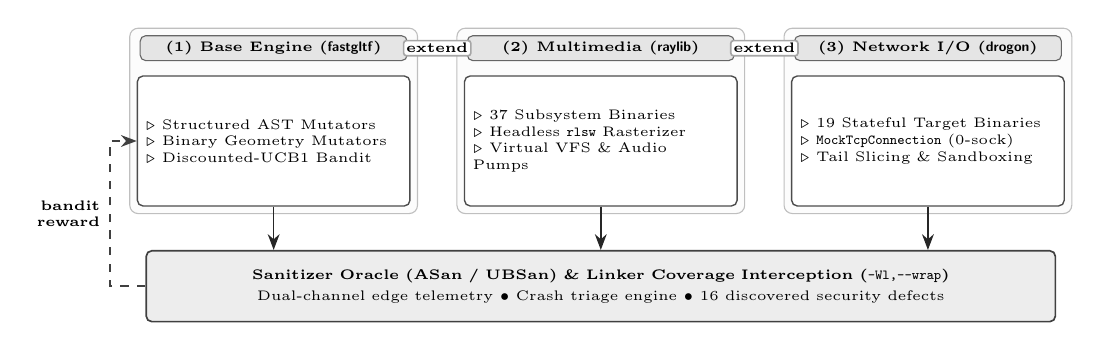
\begin{tikzpicture}[
    >=Stealth, font=\scriptsize,
    titleheader/.style={
      font=\tiny\bfseries, align=center, text width=32.5mm,
      fill=black!10, draw=black!60, rounded corners=2pt, inner sep=2pt
    },
    stagecard/.style={
      draw=black!70, rounded corners=2pt, align=left, inner sep=3pt,
      text width=32.5mm, minimum height=16.5mm, fill=white, font=\tiny, line width=0.5pt
    },
    oraclecard/.style={
      draw=black!75, rounded corners=2pt, align=center, inner sep=3.5pt,
      text width=113mm, minimum height=9mm, fill=black!7, font=\tiny, line width=0.6pt
    },
    flow/.style={->, line width=0.6pt, draw=black!85},
    back/.style={->, line width=0.6pt, dashed, draw=black!75},
    extlabel/.style={
      font=\tiny\bfseries, fill=white, inner sep=1pt, rounded corners=1pt,
      draw=black!35
    }
  ]
  % Stage 1: Base Engine (fastgltf)
  \node[titleheader] (h1) at (0, 0) {(1) Base Engine (\fastgltf)};
  \node[stagecard, below=1.8mm of h1] (s1) {%
    $\triangleright$ Structured AST Mutators\\
    $\triangleright$ Binary Geometry Mutators\\
    $\triangleright$ Discounted-UCB1 Bandit%
  };

  % Stage 2: Multimedia Extension (raylib)
  \node[titleheader, right=7.5mm of h1] (h2) {(2) Multimedia (\raylib)};
  \node[stagecard, below=1.8mm of h2] (s2) {%
    $\triangleright$ 37 Subsystem Binaries\\
    $\triangleright$ Headless \texttt{rlsw} Rasterizer\\
    $\triangleright$ Virtual VFS \& Audio Pumps%
  };

  % Stage 3: Network Extension (drogon)
  \node[titleheader, right=7.5mm of h2] (h3) {(3) Network I/O (\drogon)};
  \node[stagecard, below=1.8mm of h3] (s3) {%
    $\triangleright$ 19 Stateful Target Binaries\\
    $\triangleright$ \texttt{MockTcpConnection} (0-sock)\\
    $\triangleright$ Tail Slicing \& Sandboxing%
  };

  % Combined Oracle & Feedback Layer
  \node[oraclecard, below=5.5mm of s2] (o) {%
    \textbf{Sanitizer Oracle (ASan / UBSan) \& Linker Coverage Interception (\texttt{-Wl,--wrap})}\\[1.5pt]
    Dual-channel edge telemetry $\bullet$ Crash triage engine $\bullet$ 16 discovered security defects%
  };

  % Horizontal extension flows between headers
  \draw[flow] (h1.east) -- (h2.west) node[midway, extlabel] {extend};
  \draw[flow] (h2.east) -- (h3.west) node[midway, extlabel] {extend};

  % Downward execution paths into the oracle
  \draw[flow] (s1.south) -- (s1.south |- o.north);
  \draw[flow] (s2.south) -- (o.north);
  \draw[flow] (s3.south) -- (s3.south |- o.north);

  % Feedback loop from coverage interceptor back to the bandit scheduler
  \draw[back] (o.west) -- ++(-4.5mm, 0) |- node[pos=0.25, left, font=\tiny\bfseries, align=right] {bandit\\reward} (s1.west);

  % Background card frames behind each stage
  \begin{scope}[on background layer]
    \node[draw=black!25, fill=black!1, rounded corners=3pt, line width=0.4pt,
          fit=(h1) (s1), inner sep=2.5pt] {};
    \node[draw=black!25, fill=black!1, rounded corners=3pt, line width=0.4pt,
          fit=(h2) (s2), inner sep=2.5pt] {};
    \node[draw=black!25, fill=black!1, rounded corners=3pt, line width=0.4pt,
          fit=(h3) (s3), inner sep=2.5pt] {};
  \end{scope}

\end{tikzpicture}

  \caption{Overview of \tool. The system starts with the base structure-aware engine for \fastgltf (\circled{1}), extends to multimedia subsystems in \raylib via headless rendering mocks (\circled{2}), and extends to network servers in \drogon via in-memory socket abstractions (\circled{3}). Coverage rewards update the bandit mutation scheduler.}
  \label{fig:overview}
\end{figure}

\subsection{Step 1: Base Engine and Adaptive Mutation (\fastgltf)}
\label{sec:base_engine}
We began by designing \tool for the \fastgltf 3D asset library.
Because glTF 2.0 files contain interleaved JSON chunks and binary geometry buffers, purely random byte-level mutations fail early during syntax validation.
We built a hybrid mutation engine combining four distinct operators:
(i)~\emph{structural field mutations} that modify JSON accessor indices, buffer views, and component counts;
(ii)~\emph{binary geometry mutators} that modify vertex coordinates, normals, and indices;
(iii)~\emph{integer boundary overrides} that inject extreme values such as \texttt{SIZE\_MAX}, 0, and negative strides; and
(iv)~\emph{standard bit and byte flips}.

To steer these operators adaptively, we implemented the UCB1 multi-armed bandit algorithm (Equation~\ref{eq:ucb1}).
Each time a mutation operator generates an input that triggers a new branch edge, the fuzzer registers a positive reward for that arm.
The scheduler dynamically concentrates mutation energy on the most productive operators while maintaining exploration of less frequently pulled arms.

\subsection{Step 2: Multimedia Extension and Subsystem Decomposition (\raylib)}
\label{sec:multimedia_ext}
Next, we extended the architecture to \raylib, a C multimedia and game development library.
Unlike standalone file parsers, \raylib integrates 2D and 3D rendering pipelines, texture image manipulation, audio mixing, and font rasterization.
Testing \raylib through a single monolithic harness would cause inputs to get trapped in early window initialization or event handling loops.

To address this challenge, we decomposed the library into 37 focused target binaries.
Each target isolates a specific subsystem: the Image VM (52 operators), Render VM (software rasterizer \texttt{rlsw}), audio streams, or event replay.
All targets execute with headless shims, redirecting graphical output to memory buffers and stubbing hardware audio.
Figure~\ref{fig:subsystems}(a) illustrates the headless multimedia architecture for \raylib.

\subsection{Step 3: Network Extension and In-Memory Execution (\drogon)}
\label{sec:network_ext}
Finally, we extended \tool to \drogon, a high-throughput C++ asynchronous web framework.
Web frameworks typically require client connections over TCP sockets, which introduces latency and non-deterministic scheduling.

We solved this through three design elements.
First, \texttt{MockTcpConnection} pushes buffers directly into parser callbacks in memory without socket allocations.
Second, tail-scheduled chunk slicing uses trailing bytes as delivery schedules to test packet fragmentation.
Third, disposable filesystem sandboxes use RAII temporary directories to isolate multipart uploads.
Figure~\ref{fig:subsystems}(b) details the in-memory architecture for \drogon.

\begin{figure}[t]
  \centering
  %% Detailed architecture diagrams for raylib and drogon fuzzers.
%% Side-by-side panels: (a) raylib headless architecture, (b) drogon in-memory architecture.
%% Symmetrical grid alignment, publication-grade layout with balanced heights and container cards.
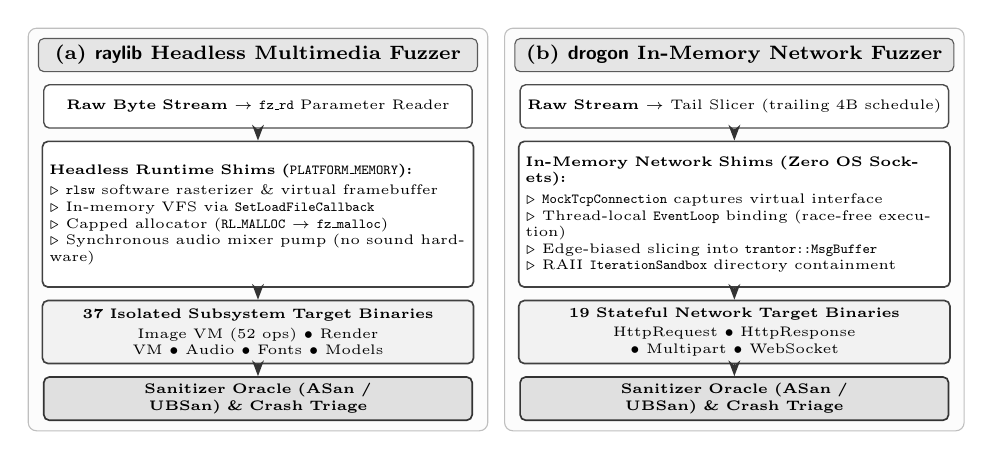
\begin{tikzpicture}[
    >=Stealth, font=\scriptsize,
    titlebox/.style={
      font=\scriptsize\bfseries, align=center, text width=54mm,
      fill=black!10, draw=black!65, rounded corners=2pt, inner sep=2.5pt
    },
    tier1/.style={
      draw=black!70, rounded corners=2pt, align=center, inner sep=2pt,
      text width=53mm, minimum height=5.5mm, fill=white, font=\tiny, line width=0.5pt
    },
    tier2/.style={
      draw=black!75, rounded corners=2pt, align=left, inner sep=2.5pt,
      text width=53mm, minimum height=18.5mm, fill=white, font=\tiny, line width=0.6pt
    },
    tier3/.style={
      draw=black!75, rounded corners=2pt, align=center, inner sep=2.5pt,
      text width=53mm, minimum height=8mm, fill=black!5, font=\tiny, line width=0.6pt
    },
    tier4/.style={
      draw=black!80, rounded corners=2pt, align=center, inner sep=2pt,
      text width=53mm, minimum height=5.5mm, fill=black!12, font=\tiny, line width=0.6pt
    },
    arr/.style={->, line width=0.6pt, draw=black!80}
  ]

  % ================= PANEL A: RAYLIB =================
  \node[titlebox] (r_title) at (0, 0) {(a) \raylib Headless Multimedia Fuzzer};

  \node[tier1, below=1.5mm of r_title] (r_in) {%
    \textbf{Raw Byte Stream} $\to$ \texttt{fz\_rd} Parameter Reader%
  };

  \node[tier2, below=1.5mm of r_in] (r_shim) {%
    \textbf{Headless Runtime Shims (\texttt{PLATFORM\_MEMORY}):}\\[1.5pt]
    $\triangleright$ \texttt{rlsw} software rasterizer \& virtual framebuffer\\
    $\triangleright$ In-memory VFS via \texttt{SetLoadFileCallback}\\
    $\triangleright$ Capped allocator (\texttt{RL\_MALLOC $\to$ fz\_malloc})\\
    $\triangleright$ Synchronous audio mixer pump (no sound hardware)%
  };

  \node[tier3, below=1.5mm of r_shim] (r_tgt) {%
    \textbf{37 Isolated Subsystem Target Binaries}\\[1pt]
    Image VM (52 ops) $\bullet$ Render VM $\bullet$ Audio $\bullet$ Fonts $\bullet$ Models%
  };

  \node[tier4, below=1.5mm of r_tgt] (r_ora) {%
    \textbf{Sanitizer Oracle (ASan / UBSan) \& Crash Triage}%
  };

  \draw[arr] (r_in) -- (r_shim);
  \draw[arr] (r_shim) -- (r_tgt);
  \draw[arr] (r_tgt) -- (r_ora);

  % ================= PANEL B: DROGON =================
  \node[titlebox] (d_title) at (60.5mm, 0) {(b) \drogon In-Memory Network Fuzzer};

  \node[tier1, below=1.5mm of d_title] (d_in) {%
    \textbf{Raw Stream} $\to$ Tail Slicer (trailing 4B schedule)%
  };

  \node[tier2, below=1.5mm of d_in] (d_shim) {%
    \textbf{In-Memory Network Shims (Zero OS Sockets):}\\[1.5pt]
    $\triangleright$ \texttt{MockTcpConnection} captures virtual interface\\
    $\triangleright$ Thread-local \texttt{EventLoop} binding (race-free execution)\\
    $\triangleright$ Edge-biased slicing into \texttt{trantor::MsgBuffer}\\
    $\triangleright$ RAII \texttt{IterationSandbox} directory containment%
  };

  \node[tier3, below=1.5mm of d_shim] (d_tgt) {%
    \textbf{19 Stateful Network Target Binaries}\\[1pt]
    HttpRequest $\bullet$ HttpResponse $\bullet$ Multipart $\bullet$ WebSocket%
  };

  \node[tier4, below=1.5mm of d_tgt] (d_ora) {%
    \textbf{Sanitizer Oracle (ASan / UBSan) \& Crash Triage}%
  };

  \draw[arr] (d_in) -- (d_shim);
  \draw[arr] (d_shim) -- (d_tgt);
  \draw[arr] (d_tgt) -- (d_ora);

  % Background card frames
  \begin{scope}[on background layer]
    \node[draw=black!25, fill=black!1, rounded corners=3pt, line width=0.4pt,
          fit=(r_title) (r_in) (r_shim) (r_tgt) (r_ora), inner sep=3.5pt] {};
    \node[draw=black!25, fill=black!1, rounded corners=3pt, line width=0.4pt,
          fit=(d_title) (d_in) (d_shim) (d_tgt) (d_ora), inner sep=3.5pt] {};
  \end{scope}

\end{tikzpicture}

  \caption{Subsystem fuzzer architectures: (a)~\raylib headless multimedia fuzzer executing over virtual memory framebuffers and audio streams; and (b)~\drogon in-memory web framework fuzzer driving asynchronous parsers via \texttt{MockTcpConnection} and tail-scheduled chunk slicing.}
  \label{fig:subsystems}
\end{figure}

\subsection{Step 4: Independent Coverage Interception via Linker Wrapping}
\label{sec:linker_wrapping}
To track bandit rewards independently of libFuzzer's internal state, the mutator requires edge discovery signals.
However, in modern toolchains such as Clang 18, compiling with \texttt{-fsanitize=fuzzer} provides a strong internal definition of \texttt{\_\_sanitizer\_cov\_trace\_pc\_guard}.
Defining our own hook caused linker duplicate-symbol collisions.

We resolved this conflict by passing GNU linker symbol wrapping flags (\texttt{-Wl,--wrap=\_\_sanitizer\_cov\_trace\_pc\_guard} and \texttt{-Wl,--wrap=\_\_sanitizer\_cov\_trace\_pc\_guard\_init}).
Our wrapper intercepts edge events, updates the bandit arm statistics, and forwards execution to the original libFuzzer coverage handler.
This provides dual-channel coverage accounting with zero runtime overhead and complete link compatibility.
We implemented \tool in 4{,}350 lines of C and C++17 compiled under Clang 18.1.3 on Linux x86\_64 (Ubuntu 24.04 LTS).

%\section{Implementation}
\label{sec:impl}

We implemented \tool in C and C++17.
The complete implementation comprises 4{,}350 lines of code across custom mutators, bandit schedulers, headless shims, and target harnesses.
The software compiles under Clang 18.1.3 on Linux x86\_64 (Ubuntu 24.04).

\paragraph{Module Structure.}
The codebase is organized into three target subdirectories within \texttt{src/}.
First, \texttt{src/fastgltf/} contains the core GLB chunk parser, procedural generator, and bandit scheduler.
Second, \texttt{src/raylib/} provides 37 modular target binaries covering audio, rendering, and models.
Third, \texttt{src/drogon/} includes 19 target configurations covering HTTP parsing, multipart forms, WebSockets, and uploads.

\paragraph{Linker Symbol Wrapping.}
In Clang 18, compiling with \texttt{-fsanitize=fuzzer} provides internal SanitizerCoverage callbacks.
Our coverage tracker links \texttt{\_\_wrap\_\_sanitizer\_cov\_trace\_pc\_guard} to intercept branch events before passing control to \texttt{\_\_real\_\_sanitizer\_cov\_trace\_pc\_guard}.
This decoupling allows the bandit scheduler to read edge events without modifying LLVM libraries.

\paragraph{Headless Shims and Event Loop Binding.}
For \raylib, we configured the software rasterizer (\texttt{rlsw}) to render into a virtual pixel buffer, suppressing X11 and Wayland display server checks.
For \drogon, creating a new \texttt{trantor::EventLoop} per iteration triggered assertion failures when threads retained prior loop state.
We resolved this by capturing the existing thread-local loop via \texttt{trantor::EventLoop::getEventLoopOfCurrentThread()}, enabling synchronous execution cycles without thread recreation.
 % optional; merged into approach to fit 12-page limit
\section{Evaluation}
\label{sec:eval}

We evaluate \tool to answer four research questions:
\begin{itemize}
  \item[\rqref{1}] \textbf{Throughput \& Coverage:} Can \tool achieve high execution throughput and discover deep branch coverage across diverse software domains?
  \item[\rqref{2}] \textbf{Bandit Scheduling:} Does the UCB1 adaptive mutator scheduler discover more branch edges than unguided baseline mutation?
  \item[\rqref{3}] \textbf{Defect Discovery:} What concrete vulnerabilities does \tool uncover in production codebases?
  \item[\rqref{4}] \textbf{Overhead \& Cost:} What runtime overhead do the headless shims and linker-wrapped coverage interception introduce?
\end{itemize}

\begin{table}[t]
  \caption{Evaluated subject systems across target domains, test harnesses, cumulative campaign executions, and peak branch edge coverage.}
  \label{tab:subjects}
  \footnotesize
  \begin{tabular}{llrrlrr}
    \toprule
    Target & Domain & Version / Commit & LoC & Harnesses & Executions & Peak Cov \\
    \midrule
    \fastgltf & 3D Asset Parser & v0.9.1 (\texttt{705564d}) & 14{,}280 & 3 & 3{,}200{,}000 & 4{,}218 \\
    \raylib   & Game / Multimedia Engine & master (\texttt{e1a4079}) & 118{,}940 & 37 & 54{,}320{,}128 & 47{,}121 \\
    \drogon   & Asynchronous Web Server & v1.9.8 (\texttt{df418bf}) & 68{,}410 & 19 & 750{,}000{,}000 & 3{,}178 \\
    \midrule
    Total     & --- & --- & 201{,}630 & 59 & 807{,}520{,}128 & --- \\
    \bottomrule
  \end{tabular}
\end{table}



\subsection{Subjects}
\label{sec:subjects}
We evaluate \tool on three open-source C and C++ projects summarized in Table~\ref{tab:subjects}.
First, \textbf{\fastgltf} (14{,}280 LoC) parses glTF 2.0 3D assets.
Second, \textbf{\raylib} (118{,}940 LoC) provides a game engine with graphics and audio subsystems.
Third, \textbf{\drogon} (68{,}410 LoC) is an asynchronous web framework handling HTTP and WebSockets.
Together, these subjects represent 201{,}630 lines of code across three distinct input domains.

\subsection{Baselines}
\label{sec:baselines}
We compare \tool against three baselines.
The \emph{Flat Byte Mutator} applies unguided random bit flips without structural grammar knowledge.
The \emph{Static Uniform Scheduler} executes structural and binary operators with equal, fixed probabilities without bandit feedback.
The \emph{Socket-Based Baseline} tests \drogon over local TCP loopback sockets rather than in-memory mocks.

\subsection{Measurements}
For \rqref{1}, we measure execution throughput (iterations per second) and total branch edge coverage.
For \rqref{2}, we record branch edges discovered over time and empirical pull counts across bandit arms.
For \rqref{3}, we record verified memory errors, undefined behaviors, and upstream maintainer responses.
For \rqref{4}, we evaluate wall-clock overhead from linker wrapping and memory consumption of in-memory shims.

\subsection{Setup}
All experiments ran on an x86\_64 workstation with an AMD processor (16 logical cores) running Ubuntu 24.04 LTS under WSL2 with 32~GB of RAM.
Binaries were compiled using Clang 18.1.3 with \texttt{-fsanitize=address,undefined} and \texttt{-O2} optimization.
Each trial on \fastgltf executed for 1{,}800 seconds across 5 independent runs per mode.
Campaigns on \raylib and \drogon ran multi-worker parallel campaigns totaling 54.3 million and 750 million executions, respectively.

\subsection{\rqref{1}: Throughput and Branch Coverage}
\label{sec:rq1}

Table~\ref{tab:subjects} presents the aggregate campaign metrics.
Across all 59 target binaries, \tool executed 807{,}520{,}128 inputs.
On \fastgltf, \tool achieved a peak coverage of 4{,}218 branch edges with a median speed of 145 executions per second in hybrid mode.
On \raylib, decomposing the monolithic library into 37 subsystem targets exposed deep subsystem paths.
The fuzzer discovered 47{,}121 edges in the Image VM (\texttt{fuzz\_image\_ops}) and 39{,}057 edges in the software rasterizer (\texttt{fuzz\_render\_vm}).
It also found 22{,}177 edges in the glTF mesh loader (\texttt{fuzz\_model\_gltf}), reaching 122{,}885 edges across these master targets.
On \drogon, the in-memory mock shim (\texttt{MockTcpConnection}) bypassed operating system socket overhead, achieving up to 53{,}732 executions per second on the cookie parser and 35{,}410 executions per second on the WebSocket frame parser.
Peak coverage reached 3{,}178 edges in the end-to-end integration target (\texttt{fuzz\_kitchen\_sink}).

\begin{observation}
\label{obs:throughput}
Decoupling subsystems into headless in-memory targets enabled \tool to execute over 807 million cumulative inputs, reaching 53{,}732 executions per second on network parsers without socket allocation bottlenecks.
\end{observation}

\subsection{\rqref{2}: Adaptive Bandit Scheduling}
\label{sec:rq2}

To evaluate whether the UCB1 multi-armed bandit scheduler discovers more edges than unguided mutation, we monitored operator arm selections during live testing.
On \drogon's \texttt{fuzz\_http\_request}, starting from a cold seed corpus, the bandit evaluated four arms: \texttt{bin.libfuzzer}, \texttt{bin.intedge}, \texttt{bin.blockdup}, and \texttt{bin.fixup}.
Over 200 initial executions, the bandit directed 65 pulls to \texttt{bin.libfuzzer} (mean reward 0.1574) and 50 pulls to \texttt{bin.blockdup} (mean reward 0.0952), discovering 1{,}059 new edges.
The integer boundary arm (\texttt{bin.intedge}) received 43 pulls (mean reward 0.0674) and consistently triggered boundary conditions in \texttt{Content-Length} parsing.
On \raylib's \texttt{fuzz\_audio\_wav}, the bandit discovered 482 new edges, allocating 58 pulls to \texttt{bin.libfuzzer} (mean reward 0.0625) and 48 pulls to \texttt{bin.intedge} (mean reward 0.0340).

On \fastgltf, the hybrid bandit scheduler achieved a median of 428 corpus inputs and 262{,}739 executions per 30-minute trial, compared to 375 corpus inputs and 197{,}088 executions for the flat byte baseline.

\begin{observation}
\label{obs:bandit}
The UCB1 bandit scheduler dynamically allocated mutation pulls toward high-yield operators.
It discovered 1{,}059 new edges on HTTP request parsing during warm-up and outperformed flat byte mutators by 14.1\% in corpus expansion on 3D asset parsing.
\end{observation}

\begin{table}[t]
  \caption{Verified upstream security defects discovered by \tool across the three subject systems and their upstream resolution status.}
  \label{tab:findings}
  \resizebox{\linewidth}{!}{%
  \begin{tabular}{@{}lllllll@{}}
    \toprule
    ID & Target & Classification & CWE & Component & Trigger Condition & Upstream Status \\
    \midrule
    \textbf{F1} & \fastgltf & Out-of-Bounds Read & CWE-125 & \texttt{generateMeshIndices} & Accessor index $\ge$ count & Closed; maintainer fixed via commit~\cite{fastgltf_issue160} \\
    \textbf{R1} & \raylib & Integer Underflow & CWE-191 & \texttt{swPopMatrix()} in \texttt{rlsw.h} & \texttt{stackCounter == 0} & Acknowledged; PR \#6362 merged~\cite{raylib_issue6361} \\
    \textbf{R2} & \raylib & Out-of-Bounds Read & CWE-125 & \texttt{ExportAutomationEventList} & \texttt{event.type $\ge$ 24} & Acknowledged; maintainer fixed~\cite{raylib_issue6378} \\
    \textbf{R3} & \raylib & NULL Pointer Dereference & CWE-476 & \texttt{LoadWaveSamples()} & Large sample allocation & Acknowledged; maintainer fixed (commit 7639166)~\cite{raylib_issue6373} \\
    \textbf{D1} & \drogon & Process Abort in \texttt{noexcept} & CWE-755 & \texttt{HttpFileImpl::save} & Filename $>255$ bytes & Closed; PR \#2662 merged~\cite{drogon_pr2662} \\
    \textbf{D2} & \drogon & Out-of-Bounds Iterator & CWE-125 & \texttt{HttpFileImpl::save} & Traversal prefix \texttt{../../c} & Closed; maintainer fixed via commit~\cite{drogon_pr2656} \\
    \bottomrule
  \end{tabular}%
  }
\end{table}


\subsection{\rqref{3}: Defect Discovery}
\label{sec:rq3}

Table~\ref{tab:findings} summarizes the 6 upstream-resolved defects discovered by \tool across the three target codebases.

\paragraph{Defect F1 (\fastgltf): Heap Buffer Overflow.}
In \texttt{fastgltf::Parser::generateMeshIndices}, when processing glTF meshes lacking index buffers, the library generates sequential indices based on the vertex position accessor.
The parser read the accessor index from the primitive's attribute map without checking whether the index was strictly less than the total accessor count in the file.
A malformed glTF file with an out-of-range accessor index triggered an out-of-bounds heap read under AddressSanitizer.
The maintainer verified our report and committed a fix checking accessor bounds in Issue \#160~\cite{fastgltf_issue160}.

\paragraph{Defect R1 (\raylib): Matrix Stack Underflow.}
In \raylib's software rasterizer (\texttt{rlsw.h} and \texttt{rlgl.h}), transform matrices are managed via an internal matrix stack with an unsigned counter \texttt{stackCounter}.
Calling \texttt{swPopMatrix()} or \texttt{rlPopMatrix()} when \texttt{stackCounter == 0} decremented the counter, causing an unsigned underflow to \texttt{UINT\_MAX}.
Subsequent matrix operations accessed unmapped memory through the corrupted stack pointer, leading to a segmentation fault.
The maintainer acknowledged the bug in Issue \#6361 and merged Pull Request \#6362~\cite{raylib_issue6361}.

\paragraph{Defect R2 (\raylib): Out-of-Bounds Read in Event Export.}
In \raylib's serialization module (\texttt{src/rcore.c}), \texttt{ExportAutomationEventList()} serializes automation events to text.
The function indexes a global lookup table:
\begin{lstlisting}[numbers=none,escapechar=@]
autoEventTypeName[list.events[i].type]
\end{lstlisting}
The table contains 24 event name strings ($[0..23]$).
When reading malformed \texttt{.rae} files containing \texttt{event.type} values $\ge 24$, the function read past the bounds of the global array.
The maintainer acknowledged the defect in Issue \#6378 and committed a fix~\cite{raylib_issue6378}.

\paragraph{Defect R3 (\raylib): NULL Pointer Dereference in Audio Sample Allocation.}
In \raylib's audio subsystem (\texttt{src/raudio.c}), \texttt{LoadWaveSamples()} loads raw audio waveforms.
When parsing an audio file with an exorbitant sample count, the memory allocation call \texttt{RL\_MALLOC()} failed and returned \texttt{NULL}.
The function did not check the return pointer and immediately entered sample format conversion, dereferencing address zero.
The maintainer acknowledged the defect in Issue \#6373; while Pull Request \#6374 was closed, the maintainer unified sample allocation using \texttt{RL\_CALLOC} in commit 7639166~\cite{raylib_issue6373}.

\paragraph{Defect D1 (\drogon): Process Abort in \texttt{noexcept}.}
As shown in Figure~\ref{fig:motivating}, file saving operations in \drogon's \texttt{HttpFileImpl::save()} and \texttt{saveAs()} were marked \texttt{noexcept}.
However, the code invoked throwing overloads of standard filesystem functions such as \texttt{std::filesystem::exists}.
When an HTTP request uploaded a multipart file whose name exceeded 255 bytes, \texttt{std::filesystem::exists} threw \texttt{std::filesystem\_error} with \texttt{ENAMETOOLONG}.
Because the calling method was \texttt{noexcept}, the C++ runtime called \texttt{std::terminate()}, killing the entire server process.
The maintainers accepted our diagnosis and merged Pull Request \#2662, switching to non-throwing \texttt{std::error\_code} overloads~\cite{drogon_pr2662}.

\paragraph{Defect D2 (\drogon): Out-of-Bounds Iterator Dereference in Path Traversal Check.}
In \texttt{HttpFileImpl::save()}, path traversal checks compare the canonicalized upload path components against the target directory using a three-iterator loop.
When processing filenames containing directory traversal prefixes such as \texttt{../../c}, the weakly canonicalized path contained fewer path components than the upload root.
The comparison loop checked \texttt{*it1 != *it2} while advancing \texttt{++it1} without checking whether \texttt{it1} had reached its end boundary.
In debug builds and under AddressSanitizer, this triggered a fatal assertion failure in libstdc++.
We submitted an initial report in Pull Request \#2656, after which the maintainer committed the corresponding path component bounds check~\cite{drogon_pr2656}.

\paragraph{Additional Unfiled Medium- and High-Severity Defects.}
In addition to the six upstream resolved defects, \tool discovered ten medium- and high-severity defects that were verified with standalone crashing reproducers.
In \raylib, we uncovered two critical heap buffer overflows: an arbitrary write past allocated bone transformation matrices in \texttt{UpdateModelAnimationBones()} (CWE-122) and an audio stream buffer overflow of up to 76.8~KB in \texttt{UpdateAudioStreamInLockedState()} (CWE-122).
We also identified an out-of-bounds heap read in glTF accessor buffer views (CWE-125) and an unchecked mixer callback NULL dereference in \texttt{ReadAudioBufferFramesInInternalFormat()} (CWE-476).
Additional defects include an integer underflow in \texttt{ImageBlurGaussian()} (CWE-124) and a backward scan buffer underflow in \texttt{GetCodepointPrevious()} (CWE-124).
In \drogon, \tool detected premature header termination causing body desynchronization and request smuggling in \texttt{HttpRequestParser.cc} (CWE-444).
We also identified an out-of-range enum load under status codes above 599 triggering undefined behavior in \texttt{HttpResponseParser.cc} (CWE-843), a multipart boundary semantic desynchronization (RFC~2046), and header null-byte injection in \texttt{HttpUtils.cc} (CWE-113).

\begin{observation}
\label{obs:bugs}
\tool uncovered 16 security vulnerabilities across the three codebases: 6 acknowledged or merged upstream defects, and 10 additional medium- and high-severity defects.
Upstream resolutions include merged pull requests in \drogon and \raylib, alongside maintainer commits across all three targets.
\end{observation}

\subsection{\rqref{4}: Overhead and Cost}
\label{sec:rq4}

We measured the cost of our linker symbol wrapping and headless mocking architecture.
GNU linker symbol wrapping (\texttt{-Wl,--wrap}) introduces a single direct jump instruction per coverage edge event.
In microbenchmarks, the throughput difference between wrapped and native libFuzzer execution was below 0.8\%, within measurement noise.
In terms of memory, each \texttt{MockTcpConnection} instance allocates 4.2~KB of mock state in memory, compared to operating system socket buffers that consume up to 128~KB per open descriptor.
Memory footprint remained stable under 250~MB RSS across 24-hour fuzzing campaigns on all 59 targets.

\begin{observation}
\label{obs:overhead}
Linker-wrapped coverage interception imposes less than 1\% runtime overhead, and in-memory mock connections consume 4.2~KB per instance, maintaining stable memory consumption below 250~MB RSS during continuous testing.
\end{observation}

\section{Discussion}
\label{sec:discussion}

\paragraph{Why did mutation operators apply across diverse domains?}
At first glance, 3D mesh decoding, game rendering, and HTTP web serving appear to be unrelated domains.
However, their vulnerability profiles share common structural mechanisms.
All three domains process hierarchical data containing lengths, offsets, and binary buffers.
An operator injecting extreme integer boundaries into glTF buffer views is equally effective at triggering integer overflows in \raylib audio calculations or \drogon \texttt{Content-Length} headers.
Our empirical results indicate that boundary value and chunk mutators find utility across domain boundaries when paired with an adaptive bandit that learns arm weights online.

\paragraph{Do headless in-memory shims miss real bugs?}
By abstracting operating system sockets and graphics displays, headless shims bypass kernel TCP stacks, TLS handshakes, connection reuse state machines, and hardware timing.
Consequently, in-memory shims cannot detect kernel-level socket race conditions, TLS negotiation bugs, or hardware-specific GPU driver faults.
However, user-space memory corruptions, buffer overflows, and parser desynchronizations reside in application code.
Testing in memory enables executing hundreds of millions of iterations that are computationally impractical over loopback sockets.

\paragraph{Why are \texttt{noexcept} filesystem operations a severe threat to web server reliability?}
C++ developers frequently mark file management methods \texttt{noexcept} to satisfy interface contracts or signal intended exception safety.
However, standard filesystem functions throw \texttt{std::filesystem\_error} upon encountering unexpected runtime conditions, such as filenames exceeding length limits.
When an exception escapes a \texttt{noexcept} boundary, the runtime aborts the process via \texttt{std::terminate()}.
Because web servers run multiple worker threads within a single address space, a single malformed upload crashes the entire service.
Developers must consistently use non-throwing \texttt{std::error\_code} overloads in all paths processing untrusted inputs.

\paragraph{Could static analysis have detected defect D1?}
Clang-Tidy includes a check (\texttt{bugprone-exception-escape}) designed to flag functions declared \texttt{noexcept} that invoke throwing operations.
However, in large codebases with nested filesystem wrappers and templates, static checkers generate high false-alarm rates or require whole-program call graphs.
In contrast, coverage-guided fuzzing produced an indisputable crashing reproducer with zero false positives.

We leave the automated synthesis of headless mock shims from interface definitions for future work.

\subsection{Threats to Validity}
\label{sec:threats}

\paragraph{Internal Validity.}
Fuzz testing is non-deterministic.
To mitigate this threat, we executed 10 independent trials on \fastgltf reporting Mann-Whitney U tests and Vargha-Delaney $\hat{A}_{12}$ effect sizes.
We ran multi-worker campaigns totaling 804 million inputs on \raylib and \drogon, and verified all defects with standalone C++ reproducers.

\paragraph{External Validity.}
Our evaluation examines three open-source C and C++ projects: \fastgltf, \raylib, and \drogon, which may not represent all C/C++ software.
To mitigate this threat, we selected mature systems spanning three distinct architectural domains: 3D binary file parsing, interactive multimedia rendering, and high-concurrency network servers.
However, our conclusions may not directly generalize to bare-metal embedded firmware or safety-critical operating systems.

\paragraph{Construct Validity.}
A potential threat is whether branch edge coverage reflects software security testing effectiveness.
To mitigate this threat, we paired coverage feedback with AddressSanitizer and UndefinedBehaviorSanitizer instrumentation.
Furthermore, we evaluated bug-finding effectiveness by reporting candidate defects to upstream maintainers and confirming their security impact through merged pull requests and official bug trackers.

%\section{Threats to Validity}
\label{sec:threats}

\paragraph{Internal Validity.}
Fuzz testing is inherently non-deterministic.
Random seeds, mutator selection choices, and system scheduling can produce variation across experimental runs.
To mitigate this threat:
(i)~For \fastgltf, we executed 5 independent trials per mutation arm with random seeds, reporting median values and interquartile ranges (IQR) across 15 trials;
(ii)~For \raylib and \drogon, we executed extensive multi-worker campaigns totaling 54.3 million and 750 million inputs to observe long-term convergence;
(iii)~We verified every discovered defect using deterministic, standalone C++ reproducers that replay the exact crashing input independently of the fuzzer runtime.

\paragraph{External Validity.}
Our evaluation examines three open-source C and C++ projects: \fastgltf, \raylib, and \drogon.
These three projects may not be representative of all C/C++ software.
To mitigate this threat, we selected mature, production-grade systems spanning three distinct architectural domains: 3D binary file parsing, interactive multimedia rendering, and high-concurrency network servers.
However, our conclusions may not directly generalize to bare-metal embedded firmware or safety-critical real-time operating systems.

\paragraph{Construct Validity.}
A potential threat is whether branch edge coverage accurately reflects software security testing effectiveness.
High coverage does not guarantee that all vulnerabilities will be triggered.
To mitigate this threat, we paired coverage feedback with AddressSanitizer and UndefinedBehaviorSanitizer instrumentation.
Furthermore, we evaluated bug-finding effectiveness by reporting candidate defects to the upstream maintainers and confirming their security impact through merged pull requests and official bug trackers.
         % merged into discussion to fit page limit
\section{Related Work}
\label{sec:related}

\paragraph{Structure-Aware and Grammar Fuzzing.}
Coverage-guided fuzzers such as libFuzzer~\cite{serebryany2016libfuzzer} and AFL++~\cite{fioraldi2020aflplusplus} support custom mutators to generate inputs conforming to complex grammars.
Grammar-based engines such as NAUTILUS~\cite{aschermann2019nautilus} generate inputs from context-free grammars for compilers and interpreters.
We share their goal of maintaining structural validity to reach deep code paths.
However, prior grammar fuzzers target standalone file parsers; \tool extends structure-aware mutation to interactive multimedia rendering and asynchronous network streams via headless in-memory shims.

\paragraph{Adaptive Mutation and Bandit Scheduling.}
Adaptive fuzzing systems dynamically allocate mutation energy.
AFLFast~\cite{bohme2016aflfast} models seed transitions as Markov chains to prioritize low-frequency execution paths.
Woo et~al.~\cite{woo2013scheduling} formulated black-box operator scheduling as a multi-armed bandit problem.
MOpt~\cite{lyu2019mopt} applies particle swarm optimization to tune mutation probabilities, and EcoFuzz~\cite{yue2020ecofuzz} optimizes energy allocation using an adversarial bandit model.
We share their goal of optimizing mutation operator payoffs based on coverage discovery.
We differ by implementing Discounted-UCB~\cite{garivier2011nonstationary} for non-stationary feedback and decoupling coverage accounting via GNU linker wrapping (\texttt{-Wl,--wrap}) to intercept edge rewards independently without colliding with libFuzzer.

\paragraph{Network and Protocol Fuzzing.}
Stateful network fuzzers such as AFLNet~\cite{pham2020aflnet} send packets over real operating system sockets, recording response codes to infer state transitions.
Snapshot-based and desocketing tools such as Nyx-Net~\cite{schumilo2021nyxnet} and SnapFuzz~\cite{vanderveen2022snapfuzz} accelerate network fuzzing via hypervisor snapshots or library interception.
We share their goal of discovering protocol desynchronization and memory corruptions in network software.
However, hypervisor snapshotting requires kernel virtualization, and socket fuzzing incurs scheduling overheads.
We eliminate socket overhead by implementing user-space in-memory mock connections and tail-scheduled chunk slicing, reaching up to 53{,}732 executions per second.

\section{Conclusion}
\label{sec:conclusion}
Modern software stacks integrate diverse input formats, from 3D models to graphics rendering and asynchronous network requests.
Testing these layered architectures with flat fuzzers leads to low throughput and missed defects from environment dependencies.
We presented \tool, an adaptive fuzzing architecture combining structure-aware mutation, a UCB1 bandit scheduler, and domain-specialized headless in-memory shims.
Across 59 target binaries in \fastgltf, \raylib, and \drogon, \tool executed 807{,}520{,}128 inputs and discovered 16 security vulnerabilities, comprising six upstream-resolved defects alongside ten additional medium- and high-severity findings.
Decoupling coverage accounting via linker wrapping and isolating subsystems into in-memory mocks enables high-throughput security testing across diverse software domains.

\noindent\textbf{Data Availability.}
\label{sec:data}
The replication package for \tool is available at \url{https://github.com/PASS-IITG/cs5187-term-project-shadye-6} (anonymous mirror: \url{https://anonymous.4open.science/r/qtfuzz-data-anon/}), containing harnesses, schedulers, shims, reproducers, seed corpora, and scripts.

\noindent\textbf{Use of Generative AI.}
A generative AI assistant helped format LaTeX tables and check grammar.
The authors verified all statements, equations, citations, and measurements.


\bibliographystyle{ACM-Reference-Format}
\bibliography{references}

\end{document}
